% ============================================================================
% Fichier  : partie1/P01_C03_risque_cartographie.tex
% Titre    : Le Risque, de la Définition à la Cartographie
% Auteur   : MINKA MI NGUIDJOÏ Thierry Emmanuel
% Version  : 1.0 -- octobre 2026
% ============================================================================
% Sources : ISO 31000:2018 (définition du risque, principes, cadre,
% processus) ; ISO/IEC 27005:2018 (dossier Normes ; remplacée en 2022) ;
% COSO ERM 2004 (résumé français du dossier Normes) et 2017 ; INTOSAI
% GUID 5100 (trois risques d'audit) ; articles A0 et A1 (incertitude
% épistémique, NEK). Échelles de cotation : convention du cours.
% ============================================================================

\chapter{Le Risque, de la Définition à la Cartographie}
\label{chap:risque}
\chaptermark{Le risque}

\epigraph{%
    « On ne maîtrise pas un risque qu'on n'a pas nommé,\\
    ni un risque qu'on ne sait pas comparer aux autres. »%
}{Principe du gestionnaire de risques}

\niveauChapitre{Fondamental}{%
    Maîtrise du Chapitre~\ref{chap:controle-interne} (contrôle interne,
    matrice des risques et des contrôles)%
}

\begin{boxobjectifs}
\begin{itemize}
    \item Définir le risque, le risque inhérent, le risque résiduel et
          l'appétence au risque.
    \item Distinguer le risque, qui porte sur les objectifs de
          l'organisation, de l'incertitude épistémique, qui porte sur ce que
          l'auditeur sait.
    \item Coter un risque en probabilité et en impact sur une échelle
          commune.
    \item Construire une cartographie des risques et un registre, et en
          déduire les priorités de traitement.
    \item Appliquer le modèle du risque d'audit (inhérent, de contrôle, de
          détection) pour dimensionner les travaux.
    \item Articuler ISO~31000, COSO~ERM et ISO/IEC~27005.
\end{itemize}
\end{boxobjectifs}

\bigskip

% ============================================================================
\section*{Question directrice : par où commencer~?}
% ============================================================================

Le comité de direction de LiZbiZ a reçu, en un mois, trois alertes~: un écart
de stock de 186~millions FCFA, des comptes d'agents partis encore actifs,
et une coupure de courant de douze heures au centre de données de Garoua.
Chaque responsable réclame la priorité pour son dossier. M.~ETEME demande à
Mme~NKENG, la contrôleuse interne~: «~Lequel est le plus grave~?~»

Elle ne peut pas répondre~: LiZbiZ n'a ni liste de ses risques, ni échelle
pour les comparer. Ce chapitre donne ces outils. Il définit le risque
(section~\ref{sec:c03-definir}), le distingue de l'incertitude de
l'auditeur (section~\ref{sec:c03-incertitude}), apprend à le coter et à le
cartographier (sections~\ref{sec:c03-coter} et~\ref{sec:c03-carto}),
présente les risques propres à l'audit (section~\ref{sec:c03-audit}) et
situe les référentiels (section~\ref{sec:c03-referentiels}).

\separateur

% ============================================================================
\section{Définir le Risque}
\label{sec:c03-definir}
% ============================================================================

\subsection{Effet de l'incertitude sur les objectifs}

\begin{boxdef}
\termecle{Risque}\index{risque}~: effet de l'incertitude sur les objectifs.
L'effet est un écart, positif ou négatif, par rapport à ce qui est attendu.
On décrit un risque par ses sources, les événements possibles, leurs
conséquences et leur vraisemblance~\cite{iso31000_2018}.
\end{boxdef}
{\small\itshape Définition reformulée d'après l'ISO~31000:2018.}

\medskip

Cette définition a deux conséquences pratiques. D'abord, un risque se
rattache toujours à un \emph{objectif}~: « le centre de Garoua tombe en
panne » n'est un risque qu'au regard d'un objectif, par exemple « suivre
les expéditions du Nord en continu ». Ensuite, un risque peut être aussi
une opportunité~; en audit, on s'intéresse surtout aux écarts défavorables.

\subsection{Les composantes d'un risque informatique}

\begin{boxdef}
\termecle{Menace}\index{menace}~: cause potentielle d'un incident (un employé
malveillant, une panne électrique, un rançongiciel).

\medskip
\termecle{Vulnérabilité}\index{vulnérabilité}~: faiblesse qu'une menace peut
exploiter (un compte non désactivé, l'absence de groupe électrogène).

\medskip
\termecle{Vraisemblance}\index{vraisemblance} ou probabilité~: chance que
l'événement se produise sur une période donnée.

\medskip
\termecle{Impact}\index{impact}~: ampleur des conséquences sur les
objectifs, en argent, en durée d'interruption, en sanction ou en image.
\end{boxdef}

\subsection{Inhérent, résiduel, appétence}

\begin{boxdef}
\termecle{Risque inhérent}\index{risque inhérent}~: niveau du risque avant
la prise en compte des contrôles.

\medskip
\termecle{Risque résiduel}\index{risque résiduel}~: niveau du risque qui
subsiste compte tenu des contrôles réellement en place et efficaces.

\medskip
\termecle{Appétence au risque}\index{appétence au risque}~: niveau de risque
que l'organisation accepte de prendre pour atteindre ses objectifs. Elle est
fixée par l'organe de gouvernance, et non par les opérationnels.
\end{boxdef}

\begin{boxalert}
\textbf{Violation typique.} Calculer le risque résiduel en tenant compte
d'un contrôle décrit dans la procédure, mais jamais testé.

\smallskip
\textbf{Règle~:} on ne réduit le risque que du fait des contrôles dont
l'efficacité est établie. Un contrôle non évalué ne réduit rien~; sa cotation
est \NEK{} tant qu'on ne l'a pas testé (Chapitre~\ref{chap:controle-interne}).
\end{boxalert}

% ============================================================================
\section{Risque et Incertitude de l'Auditeur}
\label{sec:c03-incertitude}
% ============================================================================

Le mot « incertitude » apparaît dans la définition du risque comme dans
celle de l'auditologie (Chapitre~\ref{chap:audit-auditologie}). Il ne
désigne pas la même chose.

\begin{tableaucours}{L{3.2cm}L{4.6cm}L{4.4cm}}{%
    \tableauHeader{} &
    \tableauHeader{Risque} &
    \tableauHeader{Incertitude épistémique}
}
Porte sur & Les événements futurs qui affectent les objectifs de
l'organisation & Ce que l'auditeur (ou l'organisation) sait de l'état
actuel du système \\
Nature & En partie aléatoire~: même parfaitement informé, on ne sait pas si
la panne aura lieu & Réductible~: plus de preuves réduisent l'ignorance \\
Se mesure par & Probabilité et impact & Taux d'incertitude $U$ et
entropie $H$ des réponses \\
Exemple chez LiZbiZ & Le centre de Garoua peut tomber en panne & Personne
ne sait si le groupe électrogène a été testé \\
\end{tableaucours}
\vspace{-0.8em}
\begin{center}{\small\itshape Tableau~3.1. Risque et incertitude
épistémique}\end{center}

La distinction entre composantes aléatoire et épistémique de l'incertitude
est l'une des thématiques du programme de
l'auditologie~\cite{minka2026auditologie}. Elle a une conséquence directe~:
une cartographie des risques n'est fiable que si l'on sait ce que valent les
informations qui l'alimentent. L'auditeur cote donc aussi \emph{sa
connaissance} des risques.

\begin{boxlecture}{Gestion des risques de LiZbiZ}
AUDIX CONSEIL pose dix questions sur le dispositif de gestion des risques
(existence d'une liste, d'une échelle, d'un responsable, d'un suivi…) à la
direction et aux responsables de site~: 2~\OUI{}, 3~\NON{}, 5~\NEK{}.

\medskip
\textbf{Constatation.} $\mu = 0{,}20$~; $U = 0{,}50$~; $H \approx 1{,}49$~bit.

\medskip
\textbf{Analyse} (confiance élevée). La moitié des réponses déclare ne pas
savoir~: l'organisation ignore largement comment ses risques sont gérés.
Avant de coter quoi que ce soit, il faut établir qui est responsable de
quel risque. C'est une non-conformité inconnue.

\medskip
\hfill\lecture{0{,}20}{0{,}50}{1{,}49}
\end{boxlecture}

% ============================================================================
\section{Coter un Risque}
\label{sec:c03-coter}
% ============================================================================

\subsection{Une échelle commune}

Pour comparer des risques de natures différentes, on les cote sur une même
échelle. Le cours retient une convention à quatre niveaux, courante en
pratique~; chaque organisation fixe la sienne.

\begin{tableaucours}{cL{3.6cm}L{8.0cm}}{%
    \tableauHeader{Niv.} &
    \tableauHeader{Probabilité (sur un an)} &
    \tableauHeader{Impact}
}
1 & Rare & Mineur~: perte inférieure à 5~millions FCFA, interruption de
moins de 4~heures \\
2 & Possible & Modéré~: de 5 à 50~millions FCFA, interruption de moins de
24~heures \\
3 & Probable & Majeur~: de 50 à 500~millions FCFA, interruption de 1 à
3~jours, réserve du commissaire aux comptes \\
4 & Quasi certain & Critique~: plus de 500~millions FCFA, interruption de
plus de 3~jours, sanction d'un régulateur \\
\end{tableaucours}
\vspace{-0.8em}
\begin{center}{\small\itshape Tableau~3.2. Échelles de cotation (convention
du cours)}\end{center}

Le \termecle{score}\index{score de risque} d'un risque est le produit
$\text{probabilité} \times \text{impact}$, de 1 à 16. Le risque résiduel se
calcule de la même façon, en abaissant la probabilité (ou l'impact) du
seul effet des contrôles efficaces.

\subsection{Le registre de LiZbiZ}

\begin{boxscenario}{Opération LIZBIZ. Huit risques cotés}
Mme~NKENG réunit les responsables et établit le registre suivant. La colonne
« Maîtrise » indique de combien de niveaux les contrôles \emph{testés}
abaissent la probabilité.

\medskip
\begin{tableaucours}{cL{4.6cm}ccccc}{%
    \tableauHeader{Réf.} &
    \tableauHeader{Risque} &
    \tableauHeader{P} & \tableauHeader{I} & \tableauHeader{Inh.} &
    \tableauHeader{Maîtr.} & \tableauHeader{Rés.}
}
R1 & Ajustement frauduleux du stock (cumul réception et ajustement) & 4 & 3
& 12 & 0 & 12 \\
R2 & Paiement de fournisseurs fictifs & 3 & 3 & 9 & 0 & 9 \\
R3 & Usage du compte d'un agent parti & 3 & 3 & 9 & 0 & 9 \\
R4 & Arrêt prolongé du centre de Garoua & 2 & 4 & 8 & 1 & 4 \\
R5 & Perte de données faute de sauvegarde restaurable & 2 & 4 & 8 & 0 & 8 \\
R6 & Fuite de données personnelles des clients & 2 & 3 & 6 & 1 & 3 \\
R7 & Erreurs de facturation & 3 & 2 & 6 & 1 & 4 \\
R8 & Chiffrement des serveurs par un rançongiciel & 2 & 4 & 8 & 0 & 8 \\
\end{tableaucours}

\medskip
\textbf{Appétence fixée par le conseil.} Un score résiduel de 9 ou plus est
intolérable et doit être traité sans délai~; de 5 à 8, il est traité dans
l'année~; de 1 à 4, il est accepté sous surveillance.

\medskip
\textbf{Constatation.} Trois risques sont intolérables (R1, R2, R3), deux sont
à traiter dans l'année (R5, R8), trois sont acceptés (R4, R6, R7).

\medskip
\textbf{Analyse} (confiance moyenne). Les trois risques intolérables
relèvent tous du contrôle interne (séparation des tâches, gestion des
comptes), pas de la technique~: ils confirment le diagnostic du
Chapitre~\ref{chap:controle-interne}. La coupure de Garoua, qui inquiétait
le plus le comité, est en réalité le risque le mieux maîtrisé.
\end{boxscenario}

% ============================================================================
\section{Cartographier}
\label{sec:c03-carto}
% ============================================================================

\subsection{La matrice probabilité × impact}

La \termecle{cartographie des risques}\index{cartographie des risques}
représente chaque risque par sa position dans une matrice probabilité ×
impact. Les zones de couleur traduisent l'appétence~: rouge, intolérable~;
orange, à traiter~; vert, accepté.

\noindent\begin{minipage}{\linewidth}
\begin{center}
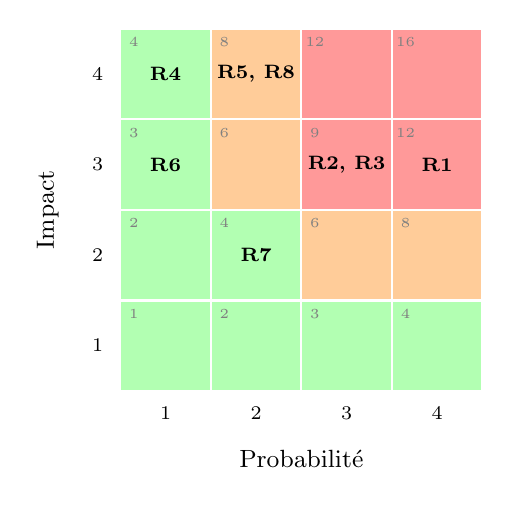
\begin{tikzpicture}[scale=1.15]
\foreach \p in {1,...,4}{
    \foreach \i in {1,...,4}{
        \pgfmathtruncatemacro{\s}{\p*\i}
        \ifnum\s>8 \def\coul{red!40}\else\ifnum\s>4 \def\coul{orange!40}\else\def\coul{green!30}\fi\fi
        \fill[\coul] (\p-1,\i-1) rectangle (\p,\i);
        \draw[white, thick] (\p-1,\i-1) rectangle (\p,\i);
        \node[font=\tiny, color=gray] at (\p-0.85,\i-0.15) {\s};
    }
}
\node[font=\scriptsize\bfseries] at (3.5,2.5) {R1};
\node[font=\scriptsize\bfseries] at (2.5,2.5) {R2, R3};
\node[font=\scriptsize\bfseries] at (1.5,3.5) {R5, R8};
\node[font=\scriptsize\bfseries] at (0.5,3.5) {R4};
\node[font=\scriptsize\bfseries] at (0.5,2.5) {R6};
\node[font=\scriptsize\bfseries] at (1.5,1.5) {R7};
\foreach \k in {1,...,4}{
    \node[font=\scriptsize] at (\k-0.5,-0.25) {\k};
    \node[font=\scriptsize] at (-0.25,\k-0.5) {\k};
}
\node[font=\small] at (2,-0.75) {Probabilité};
\node[font=\small, rotate=90] at (-0.8,2) {Impact};
\end{tikzpicture}
\end{center}
\vspace{-0.4em}
\begin{center}{\small\itshape Figure~3.1. Cartographie des risques
résiduels de LiZbiZ}\end{center}
\end{minipage}

\medskip

La cartographie se lit en trois temps~: les risques en zone rouge sont
traités en priorité~; les risques d'impact 4 restent sous surveillance même
en zone verte, car une erreur sur leur probabilité serait coûteuse~; et
l'écart entre risque inhérent et risque résiduel montre ce que les
contrôles apportent réellement.

\subsection{Traiter un risque}

Quatre options de traitement s'offrent à l'organisation~: \emph{réduire}
(ajouter ou renforcer des contrôles), \emph{transférer} (assurance,
sous-traitance, sans transférer la responsabilité), \emph{éviter} (renoncer
à l'activité) ou \emph{accepter} (dans les limites de l'appétence, par une
décision écrite).

\begin{boxprocedure}
\textbf{Le registre des risques.} Pour qu'un auditeur puisse s'appuyer sur la
cartographie, chaque ligne du registre indique~:
\begin{itemize}
    \item le risque, l'objectif menacé et son propriétaire~;
    \item la cotation inhérente, avec la justification de la probabilité et
          de l'impact~;
    \item les contrôles qui le réduisent, avec la date et le résultat de leur
          dernier test~;
    \item la cotation résiduelle et la décision de traitement~;
    \item pour un risque accepté, la décision écrite de l'instance
          compétente.
\end{itemize}
\end{boxprocedure}

\begin{boxmetier}{Responsable GRC}
\textbf{Tenir une cartographie utile}
\begin{enumerate}
    \item Faire approuver l'échelle de cotation et l'appétence par le
          conseil, avant toute cotation.
    \item Désigner un propriétaire par risque, au niveau de la direction.
    \item Ne réduire le risque résiduel que sur la base de contrôles testés.
    \item Mettre à jour la cartographie au moins une fois par an, et après
          tout incident majeur.
    \item Présenter au comité d'audit les risques en zone rouge et les
          décisions d'acceptation.
\end{enumerate}
\end{boxmetier}

\begin{boxscenario}{Opération SANAGA. Deux registres, deux échelles}
\textbf{Constatation.} La BANQUE SANAGA tient un registre des risques de
crédit et de marché, coté de 1 à 4, et la DSI un registre des risques
informatiques, coté de 1 à 5 avec d'autres critères d'impact.

\medskip
\textbf{Analyse} (confiance élevée). Le conseil ne peut pas comparer un
risque informatique à un risque de crédit, donc ne peut pas arbitrer. La
panne de mars~2026, cotée « 3 sur 5 » par la DSI, n'est jamais apparue
parmi les risques majeurs de la banque. Règle~: le risque informatique est
un risque de l'entreprise, à coter sur l'échelle commune.
\end{boxscenario}

% ============================================================================
\section{Les Risques de l'Audit}
\label{sec:c03-audit}
% ============================================================================

\subsection{Le modèle du risque d'audit}

L'auditeur court lui-même un risque~: conclure qu'une situation est
satisfaisante alors qu'elle ne l'est pas. La profession décompose ce
\termecle{risque d'audit}\index{risque d'audit} en trois éléments, que le
GUID~5100 de l'INTOSAI reprend pour l'audit des SI~\cite{intosai2019guid5100}.

\begin{boxdef}
\termecle{Risque inhérent}~(en audit)~: probabilité qu'une anomalie
significative existe, du fait de la nature même de l'activité ou du système.

\medskip
\termecle{Risque de contrôle}\index{risque de contrôle}~: probabilité que le
contrôle interne ne prévienne pas ou ne détecte pas cette anomalie.

\medskip
\termecle{Risque de détection}\index{risque de détection}~: probabilité que
les travaux de l'auditeur ne la détectent pas.
\end{boxdef}

Le modèle classique relie les trois~:
\[
    \text{RA} = \text{RI} \times \text{RC} \times \text{RD}.
\]
L'auditeur ne choisit ni le risque inhérent ni le risque de contrôle~: il
les évalue. Il choisit en revanche le risque de détection, en dimensionnant
ses tests, pour que le risque d'audit reste au niveau qu'il accepte.

\begin{boxscenario}{Opération LIZBIZ. Dimensionner les tests sur les stocks}
\textbf{Évaluation.} Risque inhérent élevé (stock de forte valeur, écart
déjà constaté), estimé à 0,9~; risque de contrôle élevé (contrôles de stock
inefficaces, Chapitre~\ref{chap:controle-interne}), estimé à 0,8. Risque
d'audit accepté~: 5~\%.

\medskip
\textbf{Calcul.} $\text{RD} = 0{,}05 / (0{,}9 \times 0{,}8) \approx 0{,}07$.

\medskip
\textbf{Analyse.} Le risque de détection doit être très faible~: AUDIX
CONSEIL ne peut pas se contenter de tester les contrôles. Il doit réaliser
des tests directs et étendus sur les données de stock
(Chapitre~\ref{chap:audit-applications}).
\end{boxscenario}

\begin{boiteRemarque}{Des probabilités vraiment mesurables~?}
Rarement. Les valeurs 0,9 ou 0,8 traduisent un jugement, pas une mesure.
Le modèle sert surtout à raisonner~: plus le risque inhérent et le risque de
contrôle sont élevés, plus les tests doivent être étendus. L'auditologie
propose d'aller plus loin en mesurant ce que l'auditeur sait réellement,
par $U$ et $H$, plutôt que de l'estimer (Chapitre~\ref{chap:conclure}).
\end{boiteRemarque}

\subsection{Un audit fondé sur les risques}

La cartographie des risques de l'organisation oriente le plan d'audit~:
on audite d'abord ce qui est le plus risqué et le moins bien connu. Le
Chapitre~\ref{chap:planifier} montrera comment passer de la cartographie au
plan d'audit.

% ============================================================================
\section{Les Référentiels du Risque}
\label{sec:c03-referentiels}
% ============================================================================

\begin{tableaucours}{L{2.8cm}L{4.4cm}L{5.0cm}}{%
    \tableauHeader{Référentiel} &
    \tableauHeader{Portée} &
    \tableauHeader{Apport}
}
ISO~31000:2018 & Tout risque, toute organisation~; non certifiable &
Principes, cadre organisationnel, processus~: contexte, appréciation
(identification, analyse, évaluation), traitement, surveillance,
communication~\cite{iso31000_2018} \\
COSO~ERM (2004, 2017) & Management des risques de l'entreprise & 2004~:
huit éléments, de l'environnement interne au pilotage~; 2017~: cinq
composantes, le risque intégré à la stratégie et à la
performance~\cite{coso2004ermfr,coso2017erm} \\
ISO/IEC~27005 & Risques liés à la sécurité de l'information & Processus
d'appréciation et de traitement, au service du SMSI de
l'ISO/IEC~27001~\cite{iso27005_2018} \\
\end{tableaucours}
\vspace{-0.8em}
\begin{center}{\small\itshape Tableau~3.3. Trois référentiels du
risque}\end{center}

\begin{boxinfo}
\textbf{Édition en vigueur.} Le dossier \texttt{Normes} du cours contient
l'ISO/IEC~27005 dans son édition de 2018. Une édition de 2022 l'a remplacée.
Avant de s'y référer dans un rapport, vérifiez toujours l'édition en
vigueur.
\end{boxinfo}

Ces référentiels convergent sur l'essentiel~: un risque se rattache à un
objectif, se cote sur une échelle commune, se traite selon une appétence
fixée par la gouvernance, et se surveille dans le temps. Les méthodes
d'analyse de risques (EBIOS Risk Manager, MEHARI, FAIR) relèvent de l'UE de
gestion des risques~; le présent cours en retient ce dont l'auditeur a
besoin.

\separateur

\begin{boxresume}
\textbf{Ce qu'il faut retenir de ce chapitre~:}
\begin{itemize}
    \item \textbf{Le risque est l'effet de l'incertitude sur les objectifs}~:
          on le rattache toujours à un objectif.
    \item \textbf{Inhérent, résiduel, appétence}~: le résiduel ne tient
          compte que des contrôles testés~; l'appétence est fixée par la
          gouvernance.
    \item \textbf{Risque et incertitude épistémique} ne se confondent pas~:
          le premier porte sur l'avenir de l'organisation, la seconde sur ce
          que l'on sait aujourd'hui.
    \item \textbf{Une échelle commune} (probabilité × impact) permet de
          comparer et d'arbitrer~; deux échelles rendent l'arbitrage
          impossible.
    \item \textbf{La cartographie} montre les priorités~; le registre en
          garde la justification.
    \item \textbf{Le risque d'audit} = inhérent × contrôle × détection~;
          l'auditeur agit sur le risque de détection en dimensionnant ses
          tests.
\end{itemize}
\end{boxresume}

\bigskip

\begin{boxexo}[title={\ding{45}\quad Exercice~3.1. Menace, vulnérabilité, impact \niveaubase}]
Pour chacun des risques R3, R5 et R8 du registre de LiZbiZ, identifiez la
menace, la vulnérabilité et l'objectif menacé, puis justifiez la cotation
d'impact au regard du Tableau~3.2.
\end{boxexo}

\begin{boxexo}[title={\ding{45}\quad Exercice~3.2. Après les contrôles \niveaumoyen}]
LiZbiZ met en place les contrôles proposés au Chapitre~\ref{chap:controle-interne}
(séparation des tâches, validation des ajustements, revue trimestrielle des
comptes). Les tests montrent qu'ils abaissent de deux niveaux la probabilité
de R1 et de R3, et d'un niveau celle de R2.
\begin{enumerate}[(a)]
    \item Recalculez les scores résiduels de R1, R2 et R3.
    \item Repositionnez ces trois risques dans la cartographie.
    \item Quels risques restent à traiter dans l'année~?
    \item Pourquoi faut-il attendre les tests avant de mettre à jour la
          cartographie~?
\end{enumerate}
\end{boxexo}

\begin{boxexo}[title={\ding{45}\quad Exercice~3.3. Une échelle commune pour la BANQUE SANAGA \niveauexpert}]
\begin{enumerate}[(a)]
    \item Proposez une échelle d'impact commune aux risques bancaires et
          informatiques, exprimée en FCFA et en durée d'interruption.
    \item Cotez sur cette échelle le risque « échec d'une migration du
          système central ».
    \item Évaluez le risque inhérent et le risque de contrôle d'un audit de
          la gestion des changements de la banque, et déduisez-en l'étendue
          des tests.
    \item Expliquez pourquoi une réponse \NEK{} sur l'existence d'un plan de
          retour arrière doit être signalée au conseil.
\end{enumerate}
\end{boxexo}

\bigskip

\begin{boxinfo}
\textbf{Transition.} Parmi les risques de LiZbiZ, trois sont intolérables et
supposent une intention~: ajuster le stock, payer des fournisseurs fictifs,
utiliser le compte d'un agent parti. Le Chapitre~\ref{chap:fraude} est
consacré à la fraude dans et par les systèmes d'information.
\end{boxinfo}
